\itemhead{习题4.2 · 第10题（教材p.114）}{XJ-B1-C04-HW-P114-Y0935}
\label{XJ-B1-C04-HW-P114-Y0935}
{\footnotesize 湘教版教材p.114 / PDF第121页 / 习题4.2 / 第10题}
\field{原题}{用图象法判断函数 $y=2^x$ 与 $y=x^2$ 的图象有几个交点，并用计算机验证。}
\field{参考答案}{有3个交点，横坐标约为 $-0.766665,2,4$。两个正根可直接代入；负根可用二分数值法定位。用作图或计算机验证时须在负半轴、正半轴均查看，不能只数2、4。}
\begin{center}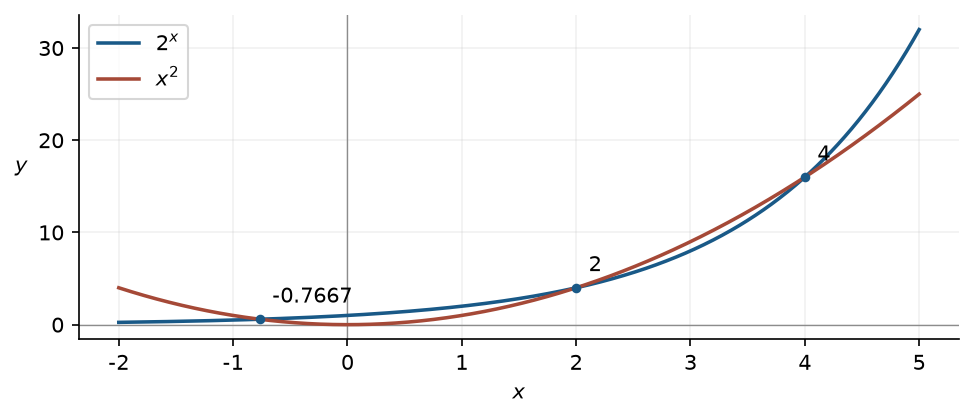
\includegraphics[width=.84\linewidth,height=.38\textheight,keepaspectratio]{figures/C04-HW114-10.png}\end{center}
{\small \field{关联知识}{F04 函数三种表示法、图象与读数（教材帮p.85、86、93、94 / PDF94、95、102、103）；E01 指数函数的概念、图象与性质（教材帮p.150、151 / PDF159、160）}
\field{方法与易错点}{把关键点与定义域一起标到图上，逐区间读交点和上下关系。 易错：将示意图预测当事实；把两曲线交点收进严格不等式；折线漏端点。}
\field{答案依据}{答案册相关题组：PDF第32页（册内页31）；按当前题库原题逐项重算，不按旧版题号机械对套。}}
